\begin{figure}[t]
\hypertarget{Figure 2}{}
\hypertarget{Panel AF2}{}
\hypertarget{Panel BF2}{}
\begin{center}
\resizebox{13.5cm}{!} {
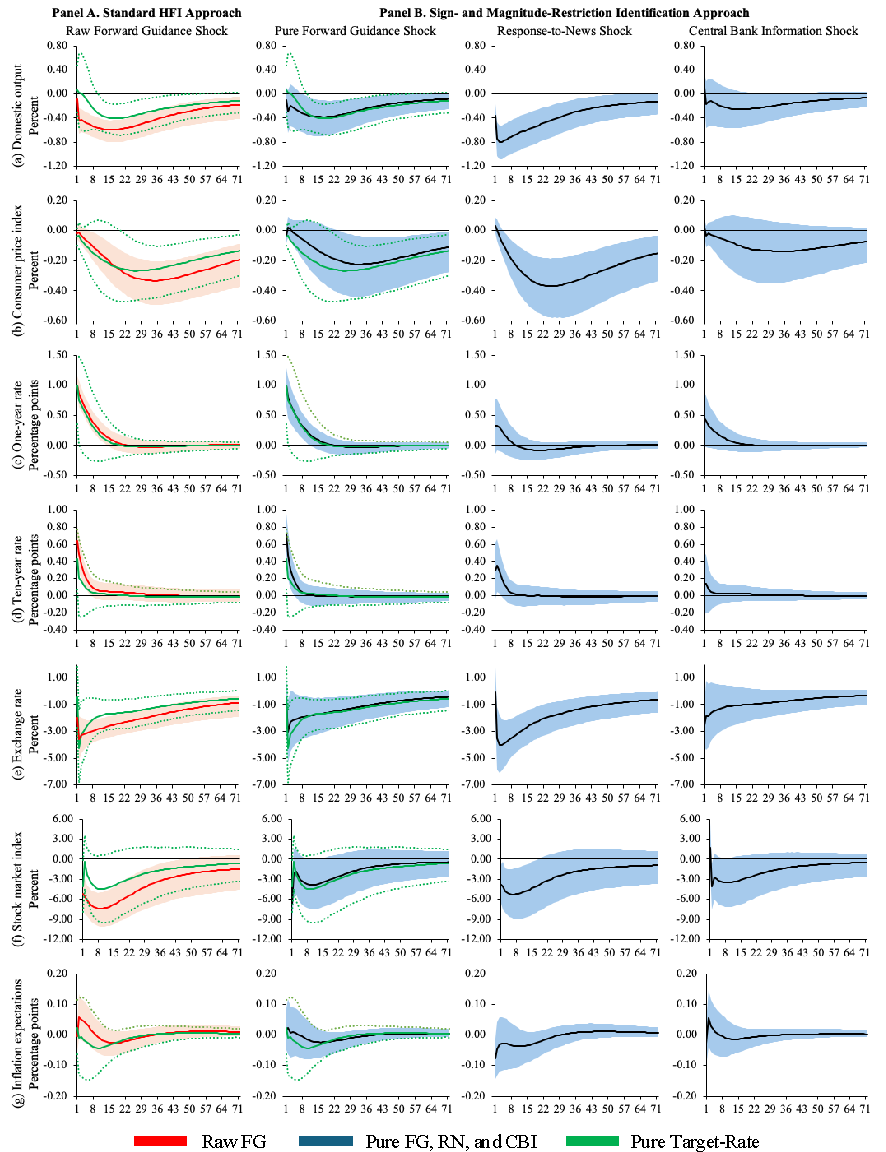
\includegraphics[width=\linewidth]{Figures/Figures_Mex/FG-2024m12_conTR-sincerores.pdf}
}
\caption[5pt]{Impulse Responses to MP, CBI, and RN shocks Disentangled from FG Surprises}
\end{center}
\begin{footnotesize} 
Notes: Responses  are  presented  for a 72-month horizon with the associated 68\% highest posterior density intervals (HPDIs). FG and target-rate shocks are normalized to imply a one percentage point increase in the one-year government bond yield. The CBI and RN shocks are scaled to match the magnitude of the normalized pure FG shock in standard deviation units.
\end{footnotesize} 
\end{figure}
